% Created 2021-03-11 Thu 14:06
% Intended LaTeX compiler: pdflatex
\documentclass[t]{beamer}
\usepackage[utf8]{inputenc}
\usepackage[T1]{fontenc}
\usepackage{graphicx}
\usepackage{grffile}
\usepackage{longtable}
\usepackage{wrapfig}
\usepackage{rotating}
\usepackage[normalem]{ulem}
\usepackage{amsmath}
\usepackage{textcomp}
\usepackage{amssymb}
\usepackage{capt-of}
\usepackage{hyperref}
\mode<beamer>{\usetheme{Amsterdam}}
\mode<beamer>{\usecolortheme{rose}}
\usepackage{fontspec}
\usepackage{polyglossia}
\setmainlanguage[babelshorthands=true]{german}
\usepackage{hyperref}
\usepackage{color}
\usepackage{xcolor}
\usepackage[misc]{ifsym}
\definecolor{darkblue}{rgb}{0,0,.5}
\definecolor{darkgreen}{rgb}{0,.5,0}
\definecolor{islamicgreen}{rgb}{0.0, 0.56, 0.0}
\definecolor{darkred}{rgb}{0.5,0,0}
\definecolor{mintedbg}{rgb}{0.95,0.95,0.95}
\definecolor{arsenic}{rgb}{0.23, 0.27, 0.29}
\definecolor{prussianblue}{rgb}{0.0, 0.19, 0.33}
\definecolor{coolblack}{rgb}{0.0, 0.18, 0.39}
\hypersetup{colorlinks=true, breaklinks=true, anchorcolor=blue,linkcolor=white, citecolor=islamicgreen, filecolor=darkred,  urlcolor=darkblue}
\usepackage{booktabs}
\usepackage{pgf}
\usepackage{minted}
\RequirePackage{fancyvrb}
\DefineVerbatimEnvironment{verbatim}{Verbatim}{fontsize=\scriptsize}
\usetheme{default}
\author{Göran Kirchner\thanks{e\_kirchnerg@doz.hwr-berlin.de}}
\date{2020-03-12}
\title{Funktionale Programmierung in F\# (2)}
\subtitle{Grundlagen \& Railway Oriented Programming}
\hypersetup{
 pdfauthor={Göran Kirchner},
 pdftitle={Funktionale Programmierung in F\# (2)},
 pdfkeywords={},
 pdfsubject={},
 pdfcreator={Emacs 27.1 (Org mode 9.4.4)}, 
 pdflang={English}}
\begin{document}

\maketitle

\section{Ziel }
\label{sec:orgd6466c9}

\begin{frame}[label={sec:orgbe70d47}]{Programm}
\begin{itemize}
\item Hausaufgaben
\item Algorithmen
\begin{itemize}
\item Operationen auf einer Liste
\item Wiederholung (Pattern Matching, Rekursion)
\end{itemize}
\item ROP (Railway Oriented Programming)
\begin{itemize}
\item Umgang mit fehlende Daten (Option)
\item Umgang mit Fehlern (Result)
\end{itemize}
\end{itemize}
\end{frame}

\section{Hausaufgaben }
\label{sec:org0e8c681}

\begin{frame}[label={sec:org888bcf8},fragile]{Two-Fer}
 \begin{minted}[bgcolor=mintedbg,frame=none,framesep=0pt,mathescape=true,fontsize=\scriptsize,breaklines=true,linenos=false,numbersep=5pt,gobble=0]{fsharp}
let twoFer (input: string option): string = 
    input 
    |> Option.defaultValue "you"
    |> sprintf "One for %s, one for me."

let test1 = [twoFer None; twoFer (Some "Alice"); twoFer (Some "Bob")]
test1
\end{minted}

\begin{verbatim}
val twoFer : input:string option -> string
val test1 : string list =
  ["One for you, one for me."; "One for Alice, one for me.";
   "One for Bob, one for me."]
\end{verbatim}
\end{frame}

\begin{frame}[label={sec:org45a545a},fragile]{Leap}
 \begin{minted}[bgcolor=mintedbg,frame=none,framesep=0pt,mathescape=true,fontsize=\scriptsize,breaklines=true,linenos=false,numbersep=5pt,gobble=0]{fsharp}
let divisible_by n d = n % d = 0
let leapYear year =
    let year_divisible_by = divisible_by year
    year_divisible_by 4
    && not(year_divisible_by 100) 
    || year_divisible_by 400

let test1 = [leapYear 1900; leapYear 1996]
let test2 = [leapYear 2000; leapYear 2019; leapYear 2020]
test1, test2
\end{minted}

\begin{verbatim}
val divisible_by : n:int -> d:int -> bool
val leapYear : year:int -> bool
val test1 : bool list = [false; true]
val test2 : bool list = [true; false; true]
\end{verbatim}
\end{frame}

\begin{frame}[label={sec:orgea0bd59},fragile]{Isogram}
 \begin{minted}[bgcolor=mintedbg,frame=none,framesep=0pt,mathescape=true,fontsize=\scriptsize,breaklines=true,linenos=false,numbersep=5pt,gobble=0]{fsharp}
let isIsogram (str: string) =
    let letters =
        str.ToLowerInvariant()
        |> Seq.filter System.Char.IsLetter
        |> Seq.toList
    letters
    |> Seq.distinct
    |> Seq.length
    |> (=) letters.Length
let test1 = [isIsogram ""; isIsogram "isogram"]
let test2 = [isIsogram "eleven"; isIsogram "subdermatoglyphic"]
test1, test2
\end{minted}

\begin{verbatim}
val isIsogram : str:string -> bool
val test1 : bool list = [true; true]
val test2 : bool list = [false; true]
\end{verbatim}
\end{frame}

\begin{frame}[label={sec:org85c498c},fragile]{Sum Of Multiples}
 \begin{minted}[bgcolor=mintedbg,frame=none,framesep=0pt,mathescape=true,fontsize=\scriptsize,breaklines=true,linenos=false,numbersep=5pt,gobble=0]{fsharp}
let multiplesOf max n =
    if n = 0 then [0] else [n .. n .. (max - 1)]
let sum (numbers: int list) (upperBound: int): int =
    numbers
    |> List.collect (multiplesOf upperBound)
    |> List.distinct
    |> List.sum
#time "on"
let test = [sum [3; 5] 1000; sum [2; 3; 5; 7; 11] 10000]
#time "off"
test
\end{minted}

\begin{verbatim}
val multiplesOf : max:int -> n:int -> int list
val sum : numbers:int list -> upperBound:int -> int
--> Timing now on
Real: 00:00:00.002, CPU: 00:00:00.002, GC gen0: 0, gen1: 0
val test : int list = [233168; 39614537]
--> Timing now off
\end{verbatim}
\end{frame}

\section{Algorithmen (List Ops) }
\label{sec:org2cccefd}
\begin{frame}[label={sec:orgb07d0f9},fragile]{length}
 \begin{minted}[bgcolor=mintedbg,frame=none,framesep=0pt,mathescape=true,fontsize=\scriptsize,breaklines=true,linenos=false,numbersep=5pt,gobble=0]{fsharp}
let rec length' list =
    match list with
    | [] -> 0
    | _::xs -> 1 + length' xs
let length list =
    let rec _length list acc =
        match list with
        | [] -> acc
        | _::xs -> _length xs (acc + 1)
    _length list 0

let test1 = [length' []; length' [1; 2; 3; 4]]
let test2 = [length []; length [1; 2; 3; 4]]
test1, test2
\end{minted}

\begin{verbatim}
val length' : list:'a list -> int
val length : list:'a list -> int
val test1 : int list = [0; 4]
val test2 : int list = [0; 4]
\end{verbatim}
\end{frame}

\begin{frame}[label={sec:orgfa6ab8e},fragile]{reverse}
 \begin{minted}[bgcolor=mintedbg,frame=none,framesep=0pt,mathescape=true,fontsize=\scriptsize,breaklines=true,linenos=false,numbersep=5pt,gobble=0]{fsharp}
let reverse list =
    let rec _reverse list acc =
        match list with
        | [] -> acc
        | x::xs -> _reverse xs (x::acc)
    _reverse list []

let test1 = reverse [1; 3; 5; 7]
let test2 = reverse [[1; 2]; [3]; []; [4..8]]
test1, test2
\end{minted}

\begin{verbatim}
val reverse : list:'a list -> 'a list
val test1 : int list = [7; 5; 3; 1]
val test2 : int list list = [[4; 5; 6; 7; 8]; []; [3]; [1; 2]]
\end{verbatim}
\end{frame}

\begin{frame}[label={sec:org6c7e644},fragile]{map}
 \begin{minted}[bgcolor=mintedbg,frame=none,framesep=0pt,mathescape=true,fontsize=\scriptsize,breaklines=true,linenos=false,numbersep=5pt,gobble=0]{fsharp}
let map f list = 
    let rec _map f list acc =
        match list with
        | [] -> acc |> reverse
        | x::xs -> _map f xs ((f x)::acc)
    _map f list []   

let test = map (fun x -> x + 1) [1; 3; 5; 7]
test
\end{minted}

\begin{verbatim}
val map : f:('a -> 'b) -> list:'a list -> 'b list
val test : int list = [2; 4; 6; 8]
\end{verbatim}
\end{frame}

\begin{frame}[label={sec:org22cceea},fragile]{filter (Übung)}
 \begin{minted}[bgcolor=mintedbg,frame=none,framesep=0pt,mathescape=true,fontsize=\scriptsize,breaklines=true,linenos=false,numbersep=5pt,gobble=0]{fsharp}
// filter : f:('a -> bool) -> list:'a list -> 'a list
let filter f list =
    ...
    match list with
    | [] -> ...
    | x::xs -> ...

let test = filter (fun x -> x % 2 = 1) [1..1000]
test
\end{minted}

\begin{verbatim}
val filter : f:('a -> bool) -> list:'a list -> 'a list
val test : int list =
  [1; 3; 5; 7; 9; 11; 13; 15; 17; 19; 21; 23; 25; 27; 29; 31; 33; 35; 37; 39;
   41; 43; 45; 47; 49; 51; 53; 55; 57; 59; 61; 63; 65; 67; 69; 71; 73; 75; 77;
   79; 81; 83; 85; 87; 89; 91; 93; 95; 97; 99; 101; 103; 105; 107; 109; 111;
   113; 115; 117; 119; 121; 123; 125; 127; 129; 131; 133; 135; 137; 139; 141;
   143; 145; 147; 149; 151; 153; 155; 157; 159; 161; 163; 165; 167; 169; 171;
   173; 175; 177; 179; 181; 183; 185; 187; 189; 191; 193; 195; 197; 199; ...]
\end{verbatim}
\end{frame}

\begin{frame}[label={sec:orga51724e},fragile]{filter (Lösung 1)}
 \begin{minted}[bgcolor=mintedbg,frame=none,framesep=0pt,mathescape=true,fontsize=\scriptsize,breaklines=true,linenos=false,numbersep=5pt,gobble=0]{fsharp}
let rec filter f list = 
    match list with
    | [] -> []
    | x::xs -> match f x with
               | true -> x :: filter f xs
               | false -> filter f xs
let test = filter (fun x -> x % 2 = 1) [1..10_000]
test
\end{minted}

\begin{verbatim}
val filter : f:('a -> bool) -> list:'a list -> 'a list
val test : int list =
  [1; 3; 5; 7; 9; 11; 13; 15; 17; 19; 21; 23; 25; 27; 29; 31; 33; 35; 37; 39;
   41; 43; 45; 47; 49; 51; 53; 55; 57; 59; 61; 63; 65; 67; 69; 71; 73; 75; 77;
   79; 81; 83; 85; 87; 89; 91; 93; 95; 97; 99; 101; 103; 105; 107; 109; 111;
   113; 115; 117; 119; 121; 123; 125; 127; 129; 131; 133; 135; 137; 139; 141;
   143; 145; 147; 149; 151; 153; 155; 157; 159; 161; 163; 165; 167; 169; 171;
   173; 175; 177; 179; 181; 183; 185; 187; 189; 191; 193; 195; 197; 199; ...]
\end{verbatim}
\end{frame}

\begin{frame}[label={sec:orge42a247},fragile]{filter (Lösung 2)}
 \begin{minted}[bgcolor=mintedbg,frame=none,framesep=0pt,mathescape=true,fontsize=\scriptsize,breaklines=true,linenos=false,numbersep=5pt,gobble=0]{fsharp}
let filter f list = 
    let rec _filter f list acc = 
        match list with
        | [] -> acc |> reverse
        | x::xs ->  match f x with
                    | true -> _filter f xs (x::acc)
                    | false -> _filter f xs acc
    _filter f list []
let test = filter (fun x -> x % 2 = 1) [1..10_000]
test
\end{minted}

\begin{verbatim}
val filter : f:('a -> bool) -> list:'a list -> 'a list
val test : int list =
  [1; 3; 5; 7; 9; 11; 13; 15; 17; 19; 21; 23; 25; 27; 29; 31; 33; 35; 37; 39;
   41; 43; 45; 47; 49; 51; 53; 55; 57; 59; 61; 63; 65; 67; 69; 71; 73; 75; 77;
   79; 81; 83; 85; 87; 89; 91; 93; 95; 97; 99; 101; 103; 105; 107; 109; 111;
   113; 115; 117; 119; 121; 123; 125; 127; 129; 131; 133; 135; 137; 139; 141;
   143; 145; 147; 149; 151; 153; 155; 157; 159; 161; 163; 165; 167; 169; 171;
   173; 175; 177; 179; 181; 183; 185; 187; 189; 191; 193; 195; 197; 199; ...]
\end{verbatim}
\end{frame}

\begin{frame}[label={sec:orgd57730c}]{Große Zahlen (Übung)}
\begin{itemize}
\item Berechne \(5^{4^{3^2}}\)
\item Wie lang ist die Zahl?
\item Gib die ersten und letzten 20 Ziffern an!
\end{itemize}
\end{frame}

\begin{frame}[label={sec:org907fe9c},fragile]{Große Zahlen (Lösung)}
 \begin{minted}[bgcolor=mintedbg,frame=none,framesep=0pt,mathescape=true,fontsize=\scriptsize,breaklines=true,linenos=false,numbersep=5pt,gobble=0]{fsharp}
#time "on"
let answer = 5I **(int (4I ** (int (3I ** 2))));;
let sans = answer.ToString()
let l = sans.Length
let prefix = sans.Substring(0,20)
let suffix = sans.Substring(l-20)
#time "off"
printfn "Length = %d, digits %s ... %s" l prefix suffix
\end{minted}

\begin{verbatim}
Real: 00:00:02.817, CPU: 00:00:02.798, GC gen0: 0, gen1: 0
val sans : string =
  "6206069878660874470748320557284679309194219265199117173177383"+[183170 chars]
val l : int = 183231
val prefix : string = "62060698786608744707"
val suffix : string = "92256259918212890625"
--> Timing now off
Length = 183231, digits 62060698786608744707 ... 92256259918212890625
\end{verbatim}
\end{frame}

\begin{frame}[label={sec:orgb972daa},fragile]{foldl}
 \begin{minted}[bgcolor=mintedbg,frame=none,framesep=0pt,mathescape=true,fontsize=\scriptsize,breaklines=true,linenos=false,numbersep=5pt,gobble=0]{fsharp}
let rec foldl folder state list = 
    match list with
    | [] -> state
    | x::xs -> foldl folder (folder state x) xs

let test1 = foldl (+) 0 [1..1_000]
let test2 = foldl (*) 1I [1I..42I]
test1, test2
\end{minted}

\begin{verbatim}
val foldl : folder:('a -> 'b -> 'a) -> state:'a -> list:'b list -> 'a
val test1 : int = 500500
val test2 : Numerics.BigInteger =
  1405006117752879898543142606244511569936384000000000
\end{verbatim}
\end{frame}

\begin{frame}[label={sec:org7523ecf},fragile]{foldr}
 \begin{minted}[bgcolor=mintedbg,frame=none,framesep=0pt,mathescape=true,fontsize=\scriptsize,breaklines=true,linenos=false,numbersep=5pt,gobble=0]{fsharp}
let flip f b a = f a b 
let rec foldr folder state list = 
    foldl (flip folder) state (reverse list)

let test = foldr (+) 5 [1; 2; 3; 4]
test
\end{minted}

\begin{verbatim}
val flip : f:('a -> 'b -> 'c) -> b:'b -> a:'a -> 'c
val foldr : folder:('a -> 'b -> 'b) -> state:'b -> list:'a list -> 'b
val test : int = 15
\end{verbatim}
\end{frame}

\begin{frame}[label={sec:orgb520d7a},fragile]{append}
 \begin{minted}[bgcolor=mintedbg,frame=none,framesep=0pt,mathescape=true,fontsize=\scriptsize,breaklines=true,linenos=false,numbersep=5pt,gobble=0]{fsharp}
let append xs ys = foldr (fun x acc -> x :: acc) ys xs

let test = append [1..5] [6..10] 
test
\end{minted}

\begin{verbatim}
val append : xs:'a list -> ys:'a list -> 'a list
val test : int list = [1; 2; 3; 4; 5; 6; 7; 8; 9; 10]
\end{verbatim}
\end{frame}

\begin{frame}[label={sec:org6c217f9},fragile]{concat (1)}
 \begin{minted}[bgcolor=mintedbg,frame=none,framesep=0pt,mathescape=true,fontsize=\scriptsize,breaklines=true,linenos=false,numbersep=5pt,gobble=0]{fsharp}
let concat xs = foldr append [] xs
let rec concat' xs = 
    match xs with
    | [] -> []
    | []::ys -> concat' ys
    | (x::xs)::ys -> x:: (concat' (xs::ys))
let concat'' xs =
    let rec _concat xs acc = 
        match xs with
        | [] -> acc |> reverse
        | []::ys -> _concat ys acc
        | (x::xs)::ys -> _concat (xs::ys) (x::acc)
    _concat xs []
\end{minted}

\begin{verbatim}
val concat : xs:'a list list -> 'a list
val concat' : xs:'a list list -> 'a list
val concat'' : xs:'a list list -> 'a list
\end{verbatim}
\end{frame}

\begin{frame}[label={sec:orgb8c7408},fragile]{concat (2)}
 \begin{minted}[bgcolor=mintedbg,frame=none,framesep=0pt,mathescape=true,fontsize=\scriptsize,breaklines=true,linenos=false,numbersep=5pt,gobble=0]{fsharp}
let test1 = concat [[1; 2]; [3]; []; [4; 5; 6]]
let test2 = concat' [[1; 2]; [3]; []; [4; 5; 6]]
let test3 = concat'' [[1; 2]; [3]; []; [4; 5; 6]]

let test1b = concat [[[1]; [2]]; [[3]]; [[]]; [[4; 5; 6]]]
let test2b = concat' [[[1]; [2]]; [[3]]; [[]]; [[4; 5; 6]]] 
let test3b = concat'' [[[1]; [2]]; [[3]]; [[]]; [[4; 5; 6]]] 
test1
\end{minted}

\begin{verbatim}
val test1 : int list = [1; 2; 3; 4; 5; 6]
val test2 : int list = [1; 2; 3; 4; 5; 6]
val test3 : int list = [1; 2; 3; 4; 5; 6]
val test1b : int list list = [[1]; [2]; [3]; []; [4; 5; 6]]
val test2b : int list list = [[1]; [2]; [3]; []; [4; 5; 6]]
val test3b : int list list = [[1]; [2]; [3]; []; [4; 5; 6]]
\end{verbatim}
\end{frame}

\begin{frame}[label={sec:org8f85440}]{Pause}
\begin{block}{}
There is no programming language, no matter how structured, 
that will prevent programmers from making bad programs.

\null\hfill--Larry Flon (1975)
\end{block}
\end{frame}

\section{ROP }
\label{sec:org65783f1}
\begin{frame}[label={sec:org66dabfa},fragile]{Option}
 \begin{minted}[bgcolor=mintedbg,frame=none,framesep=0pt,mathescape=true,fontsize=\scriptsize,breaklines=true,linenos=false,numbersep=5pt,gobble=0]{fsharp}
type BillingDetails = { 
    name : string
    billing :  string
    delivery : string option }
let order1 = {
    name = "Adam Smith"
    billing = "112 Fibonacci Street\n35813" 
    delivery = None }
let order2 = {
    name = "John Doe"
    billing = "314 Pi Avenue\n35999"
    delivery = Some "16 Planck Parkway\n62291" }
order1
\end{minted}
\end{frame}

\begin{frame}[label={sec:orgae5a9b5},fragile]{Option}
 \begin{minted}[bgcolor=mintedbg,frame=none,framesep=0pt,mathescape=true,fontsize=\scriptsize,breaklines=true,linenos=false,numbersep=5pt,gobble=0]{fsharp}
let addressForPackage (details : BillingDetails) = 
    let address =
        match details.delivery with 
        | Some s -> s
        | None -> details.billing
    sprintf "%s\n%s" details.name address
printfn "%s" (addressForPackage order1)
printfn "%s" (addressForPackage order2)
\end{minted}

\begin{verbatim}
Adam Smith
112 Fibonacci Street
35813
John Doe
16 Planck Parkway
62291
val addressForPackage : details:BillingDetails -> string
\end{verbatim}
\end{frame}

\begin{frame}[label={sec:orgfc60dca},fragile]{Option \texttt{bind} and \texttt{map}}
 \begin{minted}[bgcolor=mintedbg,frame=none,framesep=0pt,mathescape=true,fontsize=\scriptsize,breaklines=true,linenos=false,numbersep=5pt,gobble=0]{fsharp}
open System
let tryLastLine (address : string) = 
    let parts = address.Split([|'\n'|], StringSplitOptions.RemoveEmptyEntries)
    parts |> Array.tryLast
let tryPostalCode (codeString : string) = 
    match Int32.TryParse(codeString) with 
    | true, i -> i |> Some
    | false, _ -> None
let postalCodeHub (code : int) = 
    if code = 62291 then "Hub 1" else "Hub 2"
let tryHub (details : BillingDetails) = 
    details.delivery
    |> Option.bind tryLastLine 
    |> Option.bind tryPostalCode 
    |> Option.map postalCodeHub
\end{minted}
\end{frame}

\begin{frame}[label={sec:orgeb2cf63},fragile]{Option}
 \begin{minted}[bgcolor=mintedbg,frame=none,framesep=0pt,mathescape=true,fontsize=\scriptsize,breaklines=true,linenos=false,numbersep=5pt,gobble=0]{fsharp}
let test1 = order1 |> tryHub
let test2 = order2 |> tryHub
test1, test2
\end{minted}

\begin{verbatim}
(None, Some "Hub 1")
\end{verbatim}
\end{frame}

\begin{frame}[label={sec:org7b2c226}]{ROP}
\(\leadsto\) \href{./2 Railway Oriented Programming.pdf}{Railway Oriented Programming}
\end{frame}

\begin{frame}[label={sec:org097d212},fragile]{Result (Imperativ)}
 \begin{minted}[bgcolor=mintedbg,frame=none,framesep=0pt,mathescape=true,fontsize=\scriptsize,breaklines=true,linenos=false,numbersep=5pt,gobble=0]{fsharp}
open System
let checkString (s : string) =
    if isNull(s) then
        raise <| ArgumentNullException("Must not be null")
    elif String.IsNullOrEmpty(s) then
        raise <| ArgumentException("Must not be empty")
    elif String.IsNullOrWhiteSpace(s) then
        raise <| ArgumentException("Must not be white space")
    else
        s
//checkString null
//checkString ""
checkString " "
\end{minted}

\begin{verbatim}
System.ArgumentException: Must not be white space
  at FSI_0172.checkString (System.String s) [0x00046] in <fb4c844d1b764685ac9740f5612a7cfd>:0 
  at <StartupCode$FSI_0172>.$FSI_0172.main@ () [0x00000] in <fb4c844d1b764685ac9740f5612a7cfd>:0 
  at (wrapper managed-to-native) System.Reflection.RuntimeMethodInfo.InternalInvoke(System.Reflection.RuntimeMethodInfo,object,object[],System.Exception&)
  at System.Reflection.RuntimeMethodInfo.Invoke (System.Object obj, System.Reflection.BindingFlags invokeAttr, System.Reflection.Binder binder, System.Object[] parameters, System.Globalization.CultureInfo culture) [0x0006a] in <2340fc16524a4335b1ffb55cb251f8d6>:0 
Stopped due to error
\end{verbatim}
\end{frame}

\begin{frame}[label={sec:orgb56dfa1},fragile]{Result (Result<'Success,'Failure>)}
 \begin{minted}[bgcolor=mintedbg,frame=none,framesep=0pt,mathescape=true,fontsize=\scriptsize,breaklines=true,linenos=false,numbersep=5pt,gobble=0]{fsharp}
open System
let notEmpty (s : string) =
    if isNull(s) then Error "Must not be null"
    elif String.IsNullOrEmpty(s) then Error "Must not be empty"
    elif String.IsNullOrWhiteSpace(s) then Error "Must not be white space"
    else Ok s
let t1 = notEmpty null;;
let t2 = notEmpty "";;
let t3 = notEmpty " ";;
notEmpty, t1, t2, t3
\end{minted}

\begin{verbatim}
val it :
  (string -> Result<string,string>) * Result<string,string> *
  Result<string,string> * Result<string,string> =
  (<fun:it@774-8>, Error "Must not be null", Error "Must not be empty",
   Error "Must not be white space")
\end{verbatim}
\end{frame}

\begin{frame}[label={sec:orgd67faa8},fragile]{Result (Error-Types DU)}
 \begin{minted}[bgcolor=mintedbg,frame=none,framesep=0pt,mathescape=true,fontsize=\scriptsize,breaklines=true,linenos=false,numbersep=5pt,gobble=0]{fsharp}
open System
type ValidationError =
           | MustNotBeNull
           | MustNotBeEmpty
           | MustNotBeWhiteSpace
let notEmpty (s : string) =
    if isNull(s) then Error MustNotBeNull
    elif String.IsNullOrEmpty(s) then Error MustNotBeEmpty
    elif String.IsNullOrWhiteSpace(s) then Error MustNotBeWhiteSpace
    else Ok s
let t1 = notEmpty null;;
let t2 = notEmpty "";;
let t3 = notEmpty " ";;
notEmpty, t1, t2, t3
\end{minted}

\begin{verbatim}
val it :
  (string -> Result<string,ValidationError>) * Result<string,ValidationError> *
  Result<string,ValidationError> * Result<string,ValidationError> =
  (<fun:it@789-9>, Error MustNotBeNull, Error MustNotBeEmpty,
   Error MustNotBeWhiteSpace)
\end{verbatim}
\end{frame}

\begin{frame}[label={sec:org428be94},fragile]{Map}
 \begin{itemize}
\item E.map (\texttt{<\$>}): \texttt{(a->b) -> E<a> -> E<b>}
\begin{center}
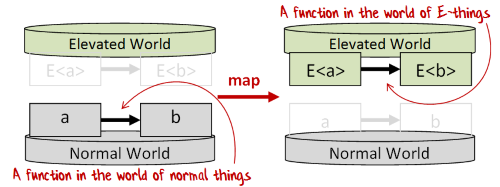
\includegraphics[width=.9\linewidth]{./../img/vgfp_map.png}
\end{center}
\begin{center}

\includegraphics[width=.9\linewidth]{./../img/vgfp_map2.png}
\end{center}
\end{itemize}
\end{frame}

\begin{frame}[label={sec:org0708048},fragile]{Bind}
 \begin{itemize}
\item E.bind (\texttt{>>=}): \texttt{(a->E<b>) -> E<a> -> E<b>}
\begin{center}
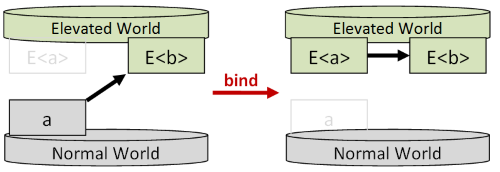
\includegraphics[width=.9\linewidth]{./../img/vgfp_bind.png}
\end{center}
\begin{center}
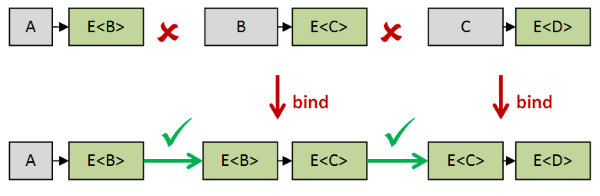
\includegraphics[width=.9\linewidth]{./../img/vgfp_bind_composition.png}
\end{center}
\end{itemize}
\end{frame}

\begin{frame}[label={sec:org85b2ee7}]{Pause}
\begin{block}{}
Applications programming is a race between software engineers, 
who strive to produce idiot-proof programs, 
and the universe which strives to produce bigger idiots. 
So far the Universe is winning.

\null\hfill-- Rick Cook (1989)
\end{block}
\end{frame}

\section{Ende }
\label{sec:org6921f9f}
\begin{frame}[label={sec:org659c59e}]{Zusammenfassung}
\begin{itemize}
\item funktionale Operationen auf Listen (Tail-Rekursion)
\item funktionaler Umgang mit fehlenden Daten (Option)
\item funktionaler Umgang mit Fehlern (Result)
\end{itemize}
\end{frame}

\begin{frame}[label={sec:orgd4abb9a}]{Links}
\begin{itemize}
\item \href{https://fsharp.org/}{fsharp.org}
\item \href{https://docs.microsoft.com/de-de/dotnet/fsharp/}{docs.microsoft.com/../dotnet/fsharp}
\item \href{https://sergeytihon.com/}{F\# weekly}
\item \href{https://fsharpforfunandprofit.com/}{fsharpforfunandprofit.com}
\item \href{https://github.com/fsprojects/awesome-fsharp}{github.com/../awesome-fsharp}
\end{itemize}
\end{frame}

\begin{frame}[label={sec:orgfe01206}]{Hausaufgabe}
\begin{itemize}
\item exercism.io (E-Mail bis 19.03)
\begin{itemize}
\item[{$\square$}] Queen Attack
\item[{$\square$}] Raindrops
\item[{$\square$}] Gigasecond
\item[{$\square$}] Bank Account
\end{itemize}

\item exercism.io (E-Mail bis 16.4)
\begin{itemize}
\item[{$\square$}] Accumulate
\item[{$\square$}] Space Age
\item[{$\square$}] Poker (Programmieraufgabe)
\end{itemize}
\end{itemize}
\end{frame}
\end{document}